\chapter{Penetration testing} \label{ch:pentesting}
This chapter details all penetration tests that were performed on the system. These were derived from the threat model created in chapter \ref{ch:threat-model}. All penetration tests are described in the format outlined below. If an aspect of the test was considered simple then one or more parts have been omitted.
\begin{itemize}
    \item \textit{Introduction}. Describes the attack vector that this penetration test will explore.
    \item \textit{Background}. Details the required background knowledge to perform and evaluate this penetration test, if any.
    \item \textit{Method}. Describes in detail how the test was performed, e.g in what environment, with what tools, what commands were used, etc.
    \item \textit{Results}. Describes the findings of the penetration test.
    \item \textit{Discussion}. This section contains a discussion about the reliability, validity, and generalizability of the results.
\end{itemize}

\section{Lab Environment} \label{ch:pentesting:lab-setup}
This section describes the lab environment and physical setup used when performing the pentests described below.

For the pentests involving the RF communication between the devices of the system specific hardware is required. Specifically, a Software Defined Radio (SDR) is required to be able to receive and transmit RF signals. The SDR used in this report is the HackRF One\footnotelink{greatscottgadgets.com/hackrf/one/}{2021-05-17} from Great Scott Gadgets\footnotelink{greatscottgadgets.com}{2021-05-17}. This is a popular and relatively cheap SDR, costing around 350 USD. Additionally, an ANT 500 antenna was used since the HackRF One does not come with an antenna. As for the physical setup, the RF transmitting devices of the system were placed relatively close to the SDR, within \texttt{10-20 cm}. This was done to increase the quality of the captures. By placing them close clean signals could be captured without increasing the gain parameters of the SDR. Figure \ref{fig:rf-lab-setup} shows a picture of the physical lab environment.
\begin{figure}[!ht]
    \centering
    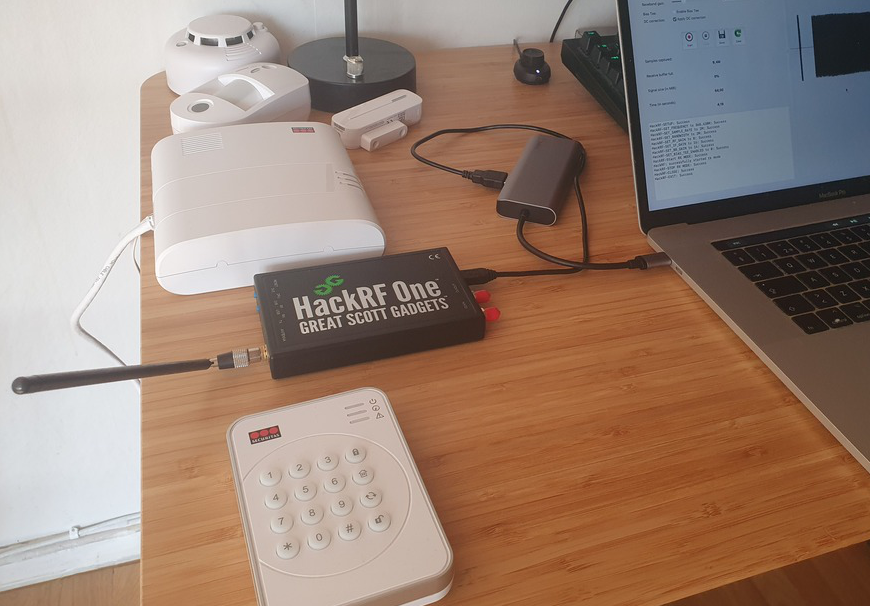
\includegraphics[width=0.9\textwidth]{images/6-pentesting/lab-setup.png}
    \caption{The lab setup used to capture and replay RF signals.}
    \label{fig:rf-lab-setup}
\end{figure}

\clearpage\section{Task 1: Replay attack on the RF communication} \label{ch:pentesting:replay}
This section details a penetration test against the RF communication between the hardware devices of the system. The specific attack vector explored in this section is a replay attack.

\subsubsection{Background}
A replay attack is an attack in network communication. The attacker listens in on the network traffic and simply retransmits the whole packets or information discovered in the packets to perform authenticated requests against a system they would otherwise not be able to. This type of vulnerability can have devastating consequences since even if several security measures have been taken, such as encrypting the data, the system can still be vulnerable to replay attacks. A replay attack is what is known as a \enquote{zero knowledge attack}, meaning the attacker needs no knowledge of how the message is structured or what it contains, and can even work on encrypted protocols \cite{hacking-the-iot-talk, rf-exploitation-talk}. This makes it often a very easy attack to perform.

Remote Keyless Entry (RKE) systems are notorious for being vulnerable to replay attacks. A famous example is RKE systems in car keys, used to unlock a car with from a distance a press of a button. When these first arrived on the market the security was extremely lacking and researchers in \citeyear{car-rke-systems} found that many cars on the market have used these insecure systems for over 20 years \cite{car-rke-systems}. Often one-way communication from the key to the car over RF signals is used with no protection at all against replay attacks. Simply capturing the RF signal and replaying it would unlock the car, allowing an attacker free access whenever they please. A simple and well-tested protection against replay attacks is sending time-stamps along with your message. If the timestamp is older than some threshold when the receiver would reject the message \cite{rke-replay}. This can, however, sometimes be difficult to implement in embedded systems since it requires both parties to agree on the time. For devices with an internet connection, this is easy thanks to the Network Time Protocol (NTP)\footnotelink{https://tools.ietf.org/html/rfc5905}{2021-05-03}. However, most low-powered simple IoT devices, such as a car key, do not have internet connectivity. A solution many modern systems used is a rolling code scheme \cite{hacking-the-iot-talk, kamkar2015drive}. Both systems keep an initially synchronized internal code $C$. When the transmitter sends a signal it includes this number and increments it internally. The receiver stores the last such number it received and checks that the number in the new signal is within some interval $[C+1, C+K]$, for some constant $K$. One usually accepts an interval of codes from the last accepted one in case a signal is lost or the button is pressed when you are outside the range of the car. If it is not within that range then the message is rejected. In practice, one might use this number to encrypt the message or use a sequence from a pre-defined pseudo-random number generator instead of an integer $C$.

This technique protects against replay attacks, however, it is still vulnerable against what is called a \textit{rolljam attack}. By jamming the signal and at the same time recording it the attacker now has a signal they can replay to have one-time access to unlock the system. Most modern cars are still susceptible to this type of attack \cite{hacking-the-iot-talk, kamkar2015drive}.

\subsubsection{Method} \label{ch:pentesting:replay:method}
The physical setup used during this test is described in section \ref{ch:pentesting:lab-setup}. As stated, a HackRF One SDR was used to receive and transmit RF signals. While low-level protocols exist to control the HackRF One, one usually uses higher-level tools to interact with it. The method of this test builds on the open-source tool \textit{Universal Radio Hacker} (URH), which was created by researchers at Hochschule Stralsund – University of Applied Sciences in Germany \cite{urh-paper}.

Initially, the center frequency at which the system communicates had to be found. This was done using the URH's \textit{Spectrum Analyzer} tool, see figure \ref{fig:finding-center-freq}. In the menu, \textit{HackRF} was selected under devices and the frequency band to listen to was selected. We know from the official documentation that the system communicates at \texttt{868 MHz} \citeyear{hsgw-user-manual}. Initially, that frequency was set in the menu options. The rest of the parameters were not important and left at their default values. To get the system to transmit data over RF communication, the tamper sensor located on the back of the door sensor was repeatedly pressed and released. While doing this, one could see a clear spike in the frequency spectrum and deduce that the center frequency used by the system is approximately \texttt{868.64 MHz}. This is clearly visible in figure \ref{fig:finding-center-freq}. The result makes sense since the frequency band \texttt{868.6–868.7 MHz} is allocated specifically for alarm systems in Europe \cite{etsi-srd-regulation}, as regulated by ETSI \footnotelink{https://www.etsi.org/}{2021-05-14}.
\begin{figure}[!ht]
    \centering
    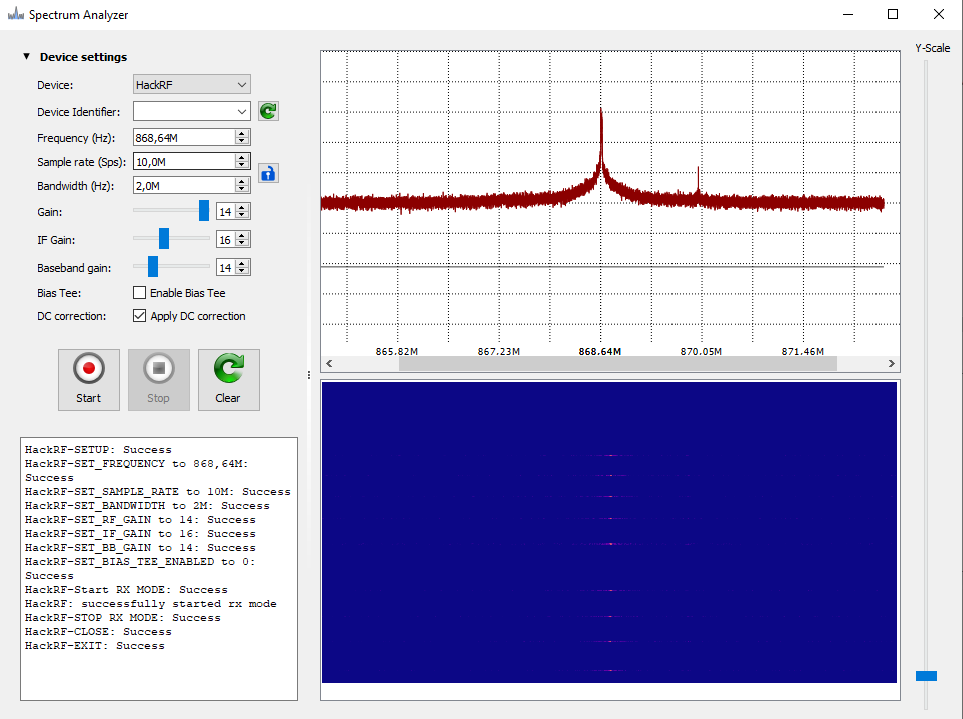
\includegraphics[width=0.9\textwidth]{images/6-pentesting/find-frequency.png}
    \caption{Finding the center frequency of the RF communication.}
    \label{fig:finding-center-freq}
\end{figure}

When the center frequency had been found, signals could be captured using URH's \textit{Record Signal} tool, see figure \ref{fig:rf-signal-capture}. This tool records raw audio signals captures from an SDR. In the menu options, one has to select the correct frequency. After some trial and error, \texttt{868.638 MHz} was found to yield well-captured signals. By placing the HackRF close to the devices, the SDR was able to capture clean signals without increasing the gain parameters. See figure \ref{fig:rf-lab-setup} for the physical setup used during this test. By zooming into the captured audio signals and seeing clear sinusoidal waves with a non-trivial pattern, one could verify that the capture was most likely done correctly. Figure \ref{fig:zoomed-in-signal} shows a magnified view of a good signal captured from the door sensor's temper alarm. This process was repeated for all identified communication endpoints of the system, capturing their signals.
\begin{figure}[!ht]
    \centering
    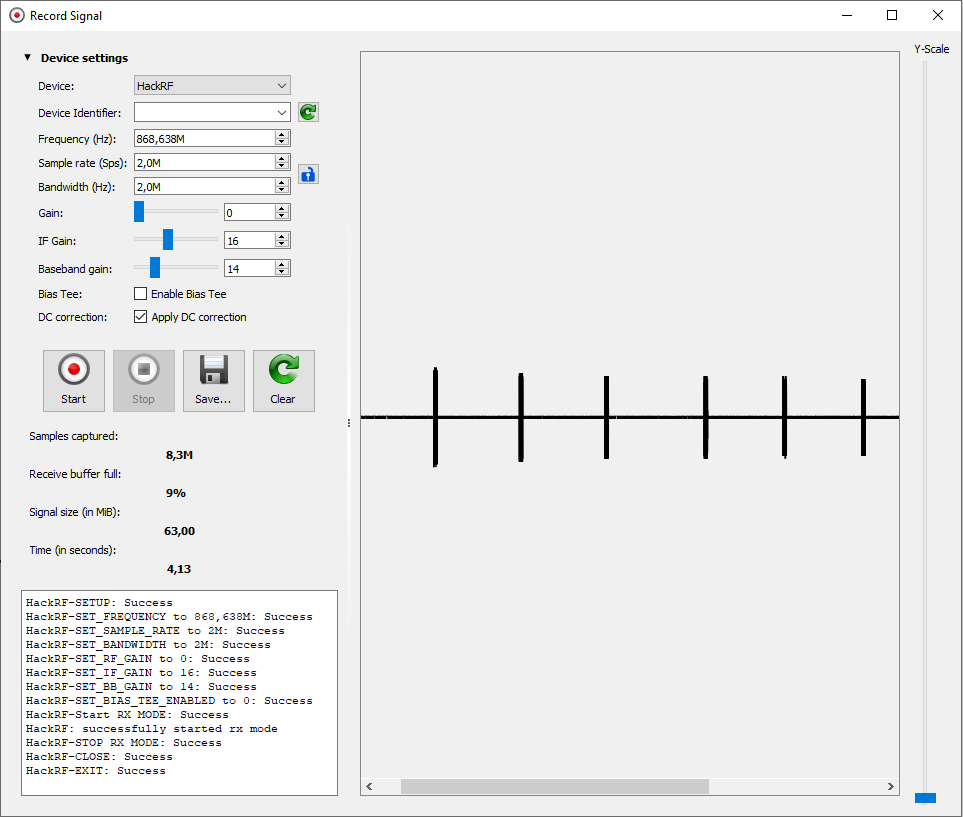
\includegraphics[width=0.9\textwidth]{images/6-pentesting/signal-capture.png}
    \caption{Capturing an RF signal using Universal Radio Hacker.}
    \label{fig:rf-signal-capture}
\end{figure}
\begin{figure}[!ht]
    \centering
    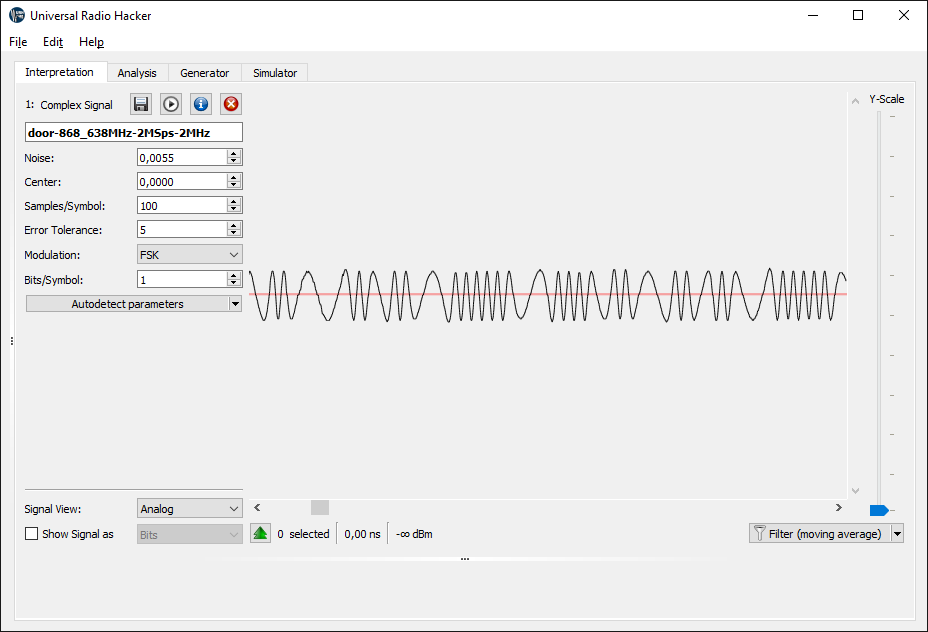
\includegraphics[width=0.9\textwidth]{images/6-pentesting/zoomed-in-signal.png}
    \caption{A cleanly captured RF signal, showing a clear sinusoidal pattern.}
    \label{fig:zoomed-in-signal}
\end{figure}

Lastly, once signals had been captured they could be replayed using URH's \textit{Send Signal} tool, see figure \ref{fig:uhr-replay-tool}. The tool lets you easily select and edit which parts of the captured signal to replay. Through a trial and error process, several combinations of packets were tested as a replay attack.
\begin{figure}[!ht]
    \centering
    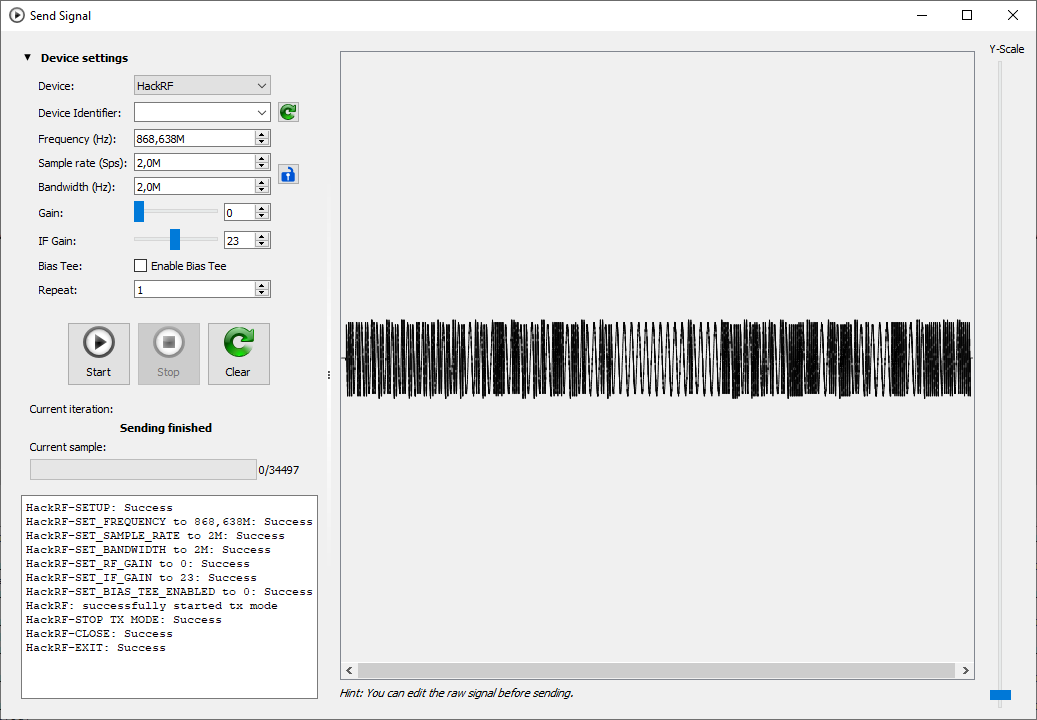
\includegraphics[width=0.9\textwidth]{images/6-pentesting/replay-signal.png}
    \caption{Performing a replay attack using Universal Radio Hacker.}
    \label{fig:uhr-replay-tool}
\end{figure}

\subsubsection{Results}
This test was successful and revealed \textit{critical} security flaws in the system. Every single tested endpoint of the RF communication was deemed vulnerable to replay attacks. The communication endpoints tested include the following:
\begin{itemize}
    \item \textbf{Arming and disarming} the alarm from the remote keypad.
    \item Triggering/resolving the tamper sensor of the door sensor.
    \item Triggering/resolving the tamper sensor of the camera.
    \item Triggering/resolving the tamper sensor of the main panel.
\end{itemize}
This has critical consequences for the security of the system. Capturing the RF signal of the user arming and disarming the alarm gives an attacker complete control of the arming state of the system. By simply replaying the signal, the main panel perceives this as a valid signal coming from the remote keypad.

\subsubsection{Discussion}
The system has no protection against replay attacks whatsoever. This conclusion is strengthened by the fact that replaying the same signals several \textit{months} later was still successful. However, replaying the signals against a different system of the same model was tested and it was unsuccessful. Presumably, some kind of ID of the device is sent making the packets invalid for another copy of the system. It clearly shows, however, that the manufacturer Climax Technology either lacks the knowledge and competence to implement secure RF communication or has decided not to prioritize security at the RF layer. Either way, this is a big mistake on their part which compromises the security of the whole system. SDRs have become much more available and much cheaper in the last few years. Attackers now have access to RF attacks which would have just a couple of years ago required very expensive and difficult to acquire hardware.

Furthermore, there are some factors that could potentially make this attack easier for an attacker in practice. When trying this attack signals were first incorrectly recorded at \texttt{868.0 MHz} instead of the correct frequency at \texttt{868.64 MHz}, giving rise to a very spiky signal. Still, the replay attack worked using this signal without issue. This indicates that perhaps the signal does not have to be captured that cleanly and that a badly captured signal, say from a distance or outside of the house, could be used to perform a replay attack. Presumably, the system implements some kind of error correction and noise filtering to increase the range and reliability of the RF communication. Additionally, regarding the tamper sensor signals, six signals are sent after one and the other, see figure \ref{fig:rf-signal-capture}. However, replaying only one of them still yields a successful replay attack. All of the six packets work individually. Presumably, the system repeats the same or similar signal several times for redundancy, in case one gets lost or corrupted in transit. This means, however, that an attacker only has to capture one of them to be able to perform a replay attack. The reliability of capturing and transmitting the signals from a distance is, however, a bit unclear. This was not tested. On the other hand, an attacker could easily purchase an RF amplifier to increase their range and sensitivity.

The consequences of this vulnerability are huge. An attack can completely bypass the alarm, defeating the whole purpose of the system in the first place. By replaying a captured disarm signal the attacker can disarm the system, granting them access to the property without triggering an alarm. Additionally, replaying any of the other signals, namely triggering the tamper sensor, an attacker could trigger an alarm of an armed system without actually entering the premises. The owner would then get a message of an active breach and security personnel would be sent to the site. One could imagine an attacker repeatedly doing this until the owner perhaps thinks the system is broken and uninstalls it, at least temporarily, from the premises. At which point the premises would no longer be protected and an attacker could strike.

\clearpage\section{Task 2: Reverse engineering the RF protocol} \label{ch:pentesting:rf-reverse-engineering}
This section covers the process of reverse engineering the RF protocol, via captured RF signals. This included mainly trying to demodulate the signals into binary data and then analyzing the contents.

\subsubsection{Background}
The system in question uses RF signals to wirelessly communicate across the devices. These radio waves are used to transfer binary data, ones and zeroes, between each device. Transferring binary data over radio waves is done by a process called modulation \cite{rf-modulation}. Digital modulation, e.g modulating binary data, is a whole field of study on to it self and that this is only a brief overview covering the basics of modulation.

There are three primary simple ways of modulating a binary signal: Amplitude- (ASK), Frequency- (FSK), and Phase- (PSK) shift keying. They each produce a distinct wave form, which can easily be visually identified. This is shown in figure \ref{fig:digital-modulation}.
\begin{figure}[!ht]
    % Perhaps I don't have the license to use this?
    \centering
    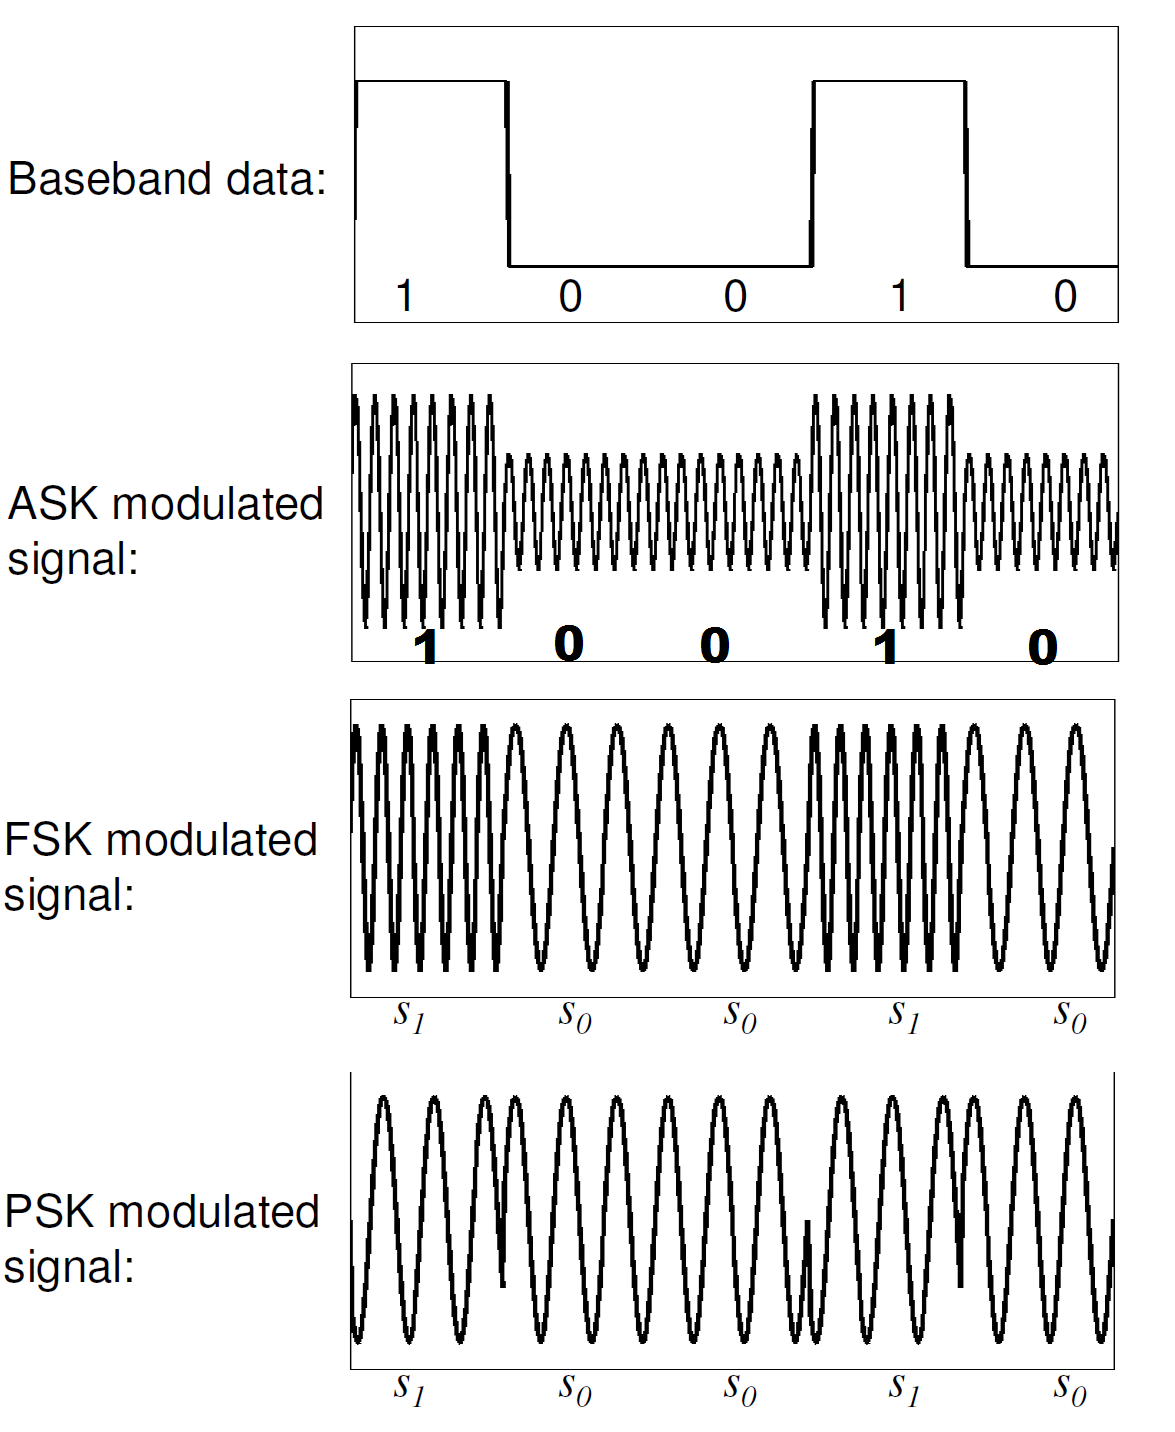
\includegraphics[width=0.7\textwidth]{images/6-pentesting/digital-modulation.png}
    \caption{The three primary techniques for digital modulation.}
    \label{fig:digital-modulation}
\end{figure}
Each technique uses a different property of the sinusoidal wave to encode a zero and one respectively. \gls{ASK} uses the amplitude of the wave, where a higher amplitude usually encodes a \texttt{1} and a lower amplitude a \texttt{0}. The frequency and phase of the wave is kept constant. \gls{FSK}, on the other hand, keeps both amplitude and phase constant. Instead two different frequencies are shifted between to differentiate between a \texttt{0} or \texttt{1}. Lastly, \gls{PSK} uses a phase-shift to differentiate between the two symbols. There are many much more complicated techniques to more efficiently encode a binary signal in radio waves \cite{rf-modulation}. However, these are not covered in this report.

Conversely, \textit{demodulation} is the process of covering a modulated signal back into the original binary data. In most real world applications of RF communication this is done directly in hardware, using specific radio receivers and circuitry to automatically convert the signal back into binary data \cite{rf-modulation}. Often this hardware also implements error correction and other techniques to increase reliability of the communication, as interference and other disturbances are unavoidable in the real world. Figure \ref{fig:bfsk-demodulator} shows a very simplified circuit that implements binary FSK (BFSK) demodulation, e.g FSK modulation using two parameter frequencies.
\begin{figure}[!ht]
    \centering
    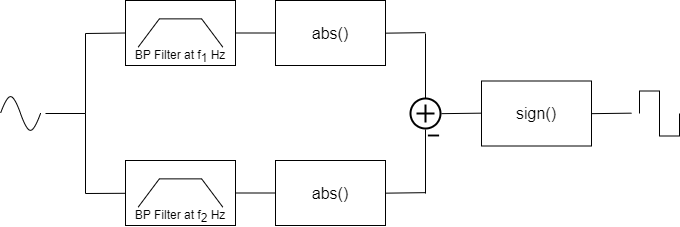
\includegraphics[width=0.8\textwidth]{images/6-pentesting/bfsk-demodulator.png}
    \caption{A simplified BFSK demodulating circuit.}
    \label{fig:bfsk-demodulator}
\end{figure}
Given a BFSK signal, modulated using the frequencies $f_1$ and $f_2$, the circuit does the following. First the signal is split and passed into two band-pass filters, tuned to the two respective parameter frequencies. Then the absolute value is applied to the signals, one of them is inverted, and they are added together. Lastly, to convert the result into the final binary wave, the signal is passed to the $sign()$ function. This circuit was inspired by material from the course \textit{EE123 Digital Signal Processing} at Berkeley EECS, specifically Lab 4 which covers FSK demodulation\footnotelink{https://sites.google.com/berkeley.edu/ee123-sp20/labs}{2021-05-18}. Demodulation can of course also be done in software, but doing so in real-time is quite CPU-intensive and consequently a lot less energy efficient. Moreover, for each modulation type there are several tuneable parameters that are hard coded in the hardware demodulation chip, such as the frequencies of the FSK modulation, which during reverse engineering have to be figured out.

\subsubsection{Method}
Initially, signals were captured according to the method described in method part of section \ref{ch:pentesting:replay:method}. Carefully inspecting the signals in \gls{URH}, as shown in figure \ref{fig:rf-signal-capture}, one can see that clearly \gls{FSK} modulation is used to modulate the signal. This conclusion is strengthened by official test documentation submitted to the \textit{Telecommunications Bureau of the Ministry of Internal Affairs and Communications} (MIC) in Japan, in which the modulation type is specified to be FSK \cite{mic-test-report}. This organization is similar to the FCC in the US. However, the information submitted to the FCC does not mention modulation type. This test document submitted to MIC was found through some extensive \gls{OSINT} and Google.

Furthermore, \gls{URH} boasts that one of their key features is automatic demodulation \cite{urh}. This was tested on all captured signals. However, it was unfortunately continuously unsuccessful to automatically find the correct parameters of the modulation. Instead, the signals were demodulated \textit{by hand} using the open source audio processing tool \textit{Audacity}\footnotelink{https://www.audacityteam.org}{2021-05-17}. The method to do this was inspired by the circuit shown in figure \ref{fig:bfsk-demodulator}, as well as an excellent tutorial by Nick Oakman, showing how to demodulate an FSK signal using Audacity \cite{oakman-fsk}. This was done in the following steps:
\begin{enumerate}
    \item The raw signal data, as captured by URH, was imported into Audacity via the menu options \texttt{File - Import - Raw Data}. URH saves the signal as raw IQ data of signed bytes. By selecting the encoding \texttt{Signed 8-bit PCM} with \texttt{2 Channels (Stereo)}, the I and Q components of the data gets imported into two separate tracks. We only care about one of them in this case and as such the stereo track was split into two mono tracks in Audacity and the second one was then deleted. The rest of the import options do not matter.

    \item Secondly, the center frequency, as perceived by Audacity, was noted. This can be found by the menu options \texttt{Analyze - Plot Spectrum}. Note that due to several features like the sample rate not being part of the raw signal data, this frequency might not equal the actual center frequency of \texttt{868.64 MHz}. This frequency was used in the steps below.

    \item A \texttt{High-Pass Filter} was applied to the first track, and a \texttt{Low-Pass Filter} to the second, with the \texttt{Roll-off} value set to \texttt{48 dB}. The former essentially maps a higher frequency to a higher amplitude in the output wave, and the latter does the opposite.

    \item Using Audacity's scripting language Nyquist\footnotelink{https://www.audacityteam.org/about/nyquist}{2021-05-17} the absolute value was applied to each track. The short Nyquist program \mintinline[style=emacs]{cl}{(s-abs *track*)} was used to do this. Then a low-pass filter was applied to both tracks, computing the envelope of the signal. Lastly, the track that originally had the low-pass filter applied to it was inverted. This means that the two tracks now corresponds to where the original signal was of high frequency and low frequency, respectively.

    \item Next the two tracks were mixed together into a new track, e.g the signals were added together.

    \item The mixed track was amplified as high as possible with clipping enabled, creating a binary signal. This created the final signal, the original binary signal, demodulated from the original signal.
    
    \item Lastly, the final binary wave was exported as raw data to a file. This was done by selecting the final track and using the menu options \texttt{File - Export - Export Selected Audio}. In the subsequent file dialog "Other uncompressed files" was selected as the type, with no heading (e.g RAW), and signed 8-bit PCM encoding. This gives you the signal as raw binary amplitude data, represented as signed bytes.
\end{enumerate}
Figure \ref{fig:audacity-demodulation} shows the process of demodulating a signal in Audacity looks like. Each track in the figure is the result of one of the steps in the above explanation.
\begin{figure}[!ht]
    \centering
    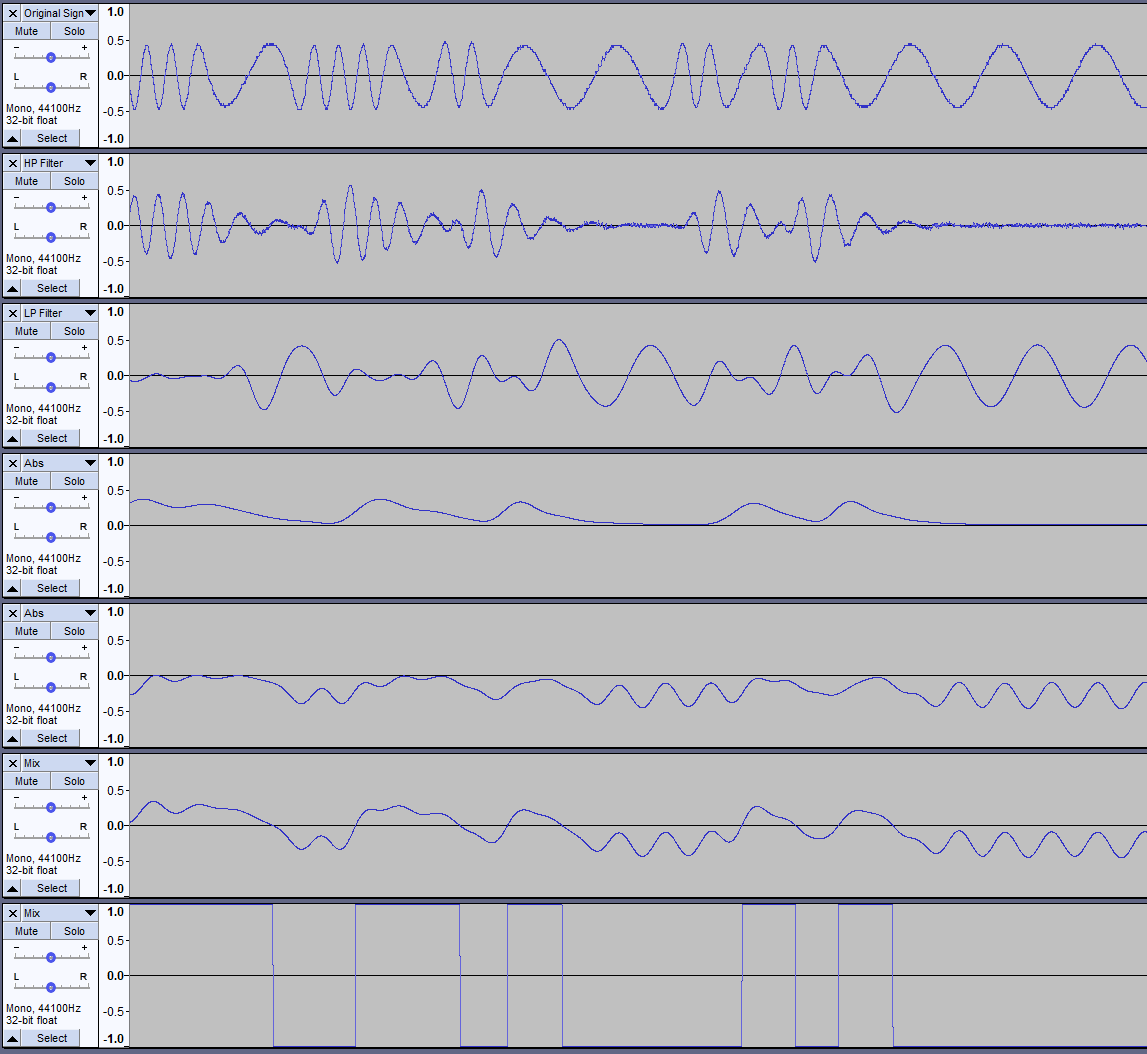
\includegraphics[width=\textwidth]{images/6-pentesting/audacity-demodulation.png}
    \caption{The process of demodulating a BFSK signal in Audacity.}
    \label{fig:audacity-demodulation}
\end{figure}
This process was applied to all captured signals. However, the result of this process is a binary wave, not the actual binary data. To extract the binary data a simple python program was created, see listing \ref{lst:extract-bits}. The program expects a list of x-axis offsets, where the first bit of the signal is. These values were found by hand, by manually looking at the plot that the program creates. The signal length and symbol length were also measured by hand, however, these are constant for all measured signals. Only the signal start offsets had to be manually derived for each signal.
\begin{figure}[ht]
    \begin{minted}[fontsize=\footnotesize, frame=single]{python}
import matplotlib.pyplot as plt

SIGNAL_LEN, SYMBOL_LEN = 34000, 200
FILE, SIGNAL_OFFSETS = "door-signal.raw", [1800, 856160, ...]

with open(FILE, "rb") as f:
  signal = [b if b < 128 else b - 256 for b in f.read()]

for i, offset in enumerate(SIGNAL_OFFSETS):
  xs = range(offset, offset + SIGNAL_LEN, SYMBOL_LEN)
  plt.scatter(xs, [0 for _ in xs], c="red")
  bits = "".join(['1' if signal[x] > 0 else '0' for x in xs])
  print(f"Packet {str(i).ljust(2)} =", hex(int(bits, 2)))

plt.plot(signal)
plt.show()
    \end{minted}
    \caption{A program to extract bits from a binary wave and plot it.}
    \label{lst:extract-bits}
\end{figure}

\subsubsection{Results}
By using the Audacity and the method described, binary data was extracted from each recorded signal. This is presented in table \ref{tb:demodulated-data}, in hexadecimal form.
\begin{table}[!ht]
    \centering
    \begin{tabularx}{\textwidth}{l}
        \hline
        \textbf{Door tamper sensor on} \\ \hline
        \texttt{0xaaaaaaaa29cd29cd0a000015d477e072b922530064} \\
        \texttt{0xaaaaaaaa29cd29cd0a0000028648b07e291d2ceecc} \\
        \texttt{0xaaaaaaaa29cd29cd0a0000280b9d2e1d2d2ca7f31c} \\
        \texttt{0xaaaaaaaa29cd29cd0a00002548c662f2feeea7fe22} \\
        \texttt{0xaaaaaaaa29cd29cd0a000019201db301398d538674} \\
        \texttt{0xaaaaaaaa29cd29cd0a00000806d6a5ee37481e2f76} \\
        \hline
        
        \textbf{Door tamper sensor off} \\ \hline
        \texttt{0xaaaaaaaa29cd29cd0a0000102366a5cb78d61c0d0c} \\
        \texttt{0xaaaaaaaa29cd29cd0a00000a3b2cb0867bf62aa616} \\
        \texttt{0xaaaaaaaa29cd29cd0a000028fe2271f089a9e8c984} \\
        \texttt{0xaaaaaaaa29cd29cd0a00001e23195bcbe8c65107ec} \\
        \texttt{0xaaaaaaaa29cd29cd0a00001913b1ee7e3448da1cf0} \\
        \texttt{0xaaaaaaaa29cd29cd0a000006f69dbb732deb2a120c} \\
        \hline
        
        \textbf{Camera tamper sensor off} \\ \hline
        \texttt{0x155555554539a539a14000034164758f44cfae66f1} \\
        \texttt{0x155555554539a539a14000034164758f44cfae66f1} \\
        \texttt{0x155555554539a539a14000034164758f44cfae66f1} \\
        \hline
    \end{tabularx}
    \caption{Binary data extracted from demodulating RF signals.}
    \label{tb:demodulated-data}
\end{table}
Analyzing the data one can see a very clear structure emerging. All recorded signals decoded into exactly 170 bits and seemingly always have the following structure:
\begin{enumerate}
    \item A preamble of alternating ones and zeroes. This is a very common technique in RF protocol to notify of an incoming signal, and to sync clock frequencies (\todo source).
    \item A sequence of bytes that is constant for each device. E.g the door sensor will always send the same byte sequence, the camera another one etc. Presumably, this is some kind of ID to tell the main panel from where the signal originates.
    \item A sequence of zero bits.
    \item A sequence of seemingly random bits. Presumably, this is the payload of the message and some kind of encryption or obfuscation is applied.
\end{enumerate}

\subsubsection{Discussion}
The signals were successfully demodulated using the described method. Data extracted from this process shows a clear structure to the messages, giving further indication that the demodulation was done correctly. By visually inspecting the signals one could see that FSK modulation was used. Additionally, this is actually documented in the official user manual \cite{hsgw-user-manual}, meaning we can be sure that this conclusion was correct. Furthermore, the signals follow patterns and standards in RF communication, such as starting with a preamble of alternating symbols, and seem to send some kind of ID to identify themselves in the protocol. This further indicates that the demodulation was done correctly.

However, the payload is clearly encrypted or at least obfuscated in some way. This is in line with the documentation provided by Climax Technology, in which they reference a \enquote{Private Encryption Method} used in the RF communication \cite{hsgw-user-manual}. What the actual method is and whether or not it is a cryptographically secure method is left unanswered. Without access to the firmware or additional documentation about the RF protocol, further reverse engineering is next to impossible given the black box state of the RF protocol.

In conclusion, this pentest did not yield any additional actionable information. While the demodulated data definitely gives some insight into the system, it does not indicate any further vulnerabilities. Trying to reverse engineer the encryption method would yield a lot of additional information, and allow an attacker to create new messages from scratch. However, without access to the firmware this is quite difficult. This is left as future work.

\clearpage\section{Task 3: RF Jamming Attack}\label{ch:pentesting:rf-jamming}
This section covers a pentest of a jamming attack against the RF communication in the system. This is a \gls{DOS} attack which if successful blocks or interferes with the RF communication between two devices, making them unable to send messages to each other \cite{hacking-the-iot-talk}.

\subsubsection{Background}
Many wireless communication mediums are vulnerable to jamming attacks. Radio frequency communication is certainly one of them. In the case of RF communication, this can be likened to a \gls{DOS} attack \cite{hacking-the-iot-talk}. A jamming attack against RF communication involves directing electromagnetic energy in one or more radio frequencies against a system to disrupt or prevent signals from being transmitted between two systems \cite{adamy2004ew}. In practice, this means sending out signals on a specific frequency, carrying enough energy to overpower anyone transmission in the same frequency band. By continuously sending out signals, such that the wireless band is filled, legitimate traffic can be blocked. Since RF communication uses a shared medium, this is an attack vector that can be incredibly hard to protect against. Often a system will communicate on a single, fixed frequency which can make the system particularly vulnerable to jamming attacks \cite{jamming-feasibility}. While many sophisticated techniques to detect jamming have been developed, detection and reporting are about the extent to which a system can react to a jamming attack \cite{optimal-jamming-defense}. Little else can usually be done, except to which frequency band or fall back to an alternate mode of communication.

\subsubsection{Method}
To transmit signals the HackRF SDR was used. It was placed close to the system, within \texttt{10-20 cm}. See section \ref{ch:pentesting:lab-setup} for a detailed description of the lab setup. To generate a jamming signal the open-source program \textit{GnuRadio Companion}\footnotelink{https://www.gnuradio.org/}{2021-05-22}, version \texttt{3.9.0.0}, was used. This is a graphical tool used to control an SDR. It is based on creating flowgraphs of connected components to receive, process, modify, and transmit real-time radio signals from and to an SDR.
\begin{figure}[!ht]
    \centering
    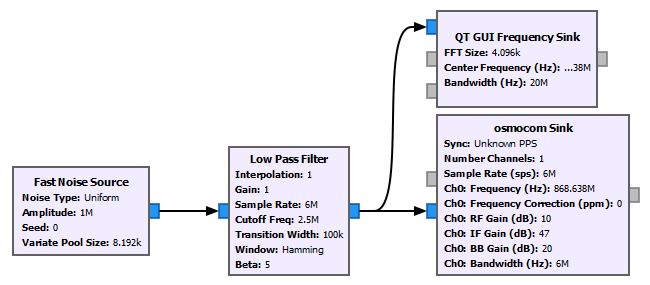
\includegraphics[width=\textwidth]{images/6-pentesting/jamming-flowgraph.png}
    \caption{A flowgraph in GnuRadio which performs a jamming attack.}
    \label{fig:gnuradio-jamming-flowgraph}
\end{figure}

To generate a noise signal, a flowgraph was created in GnuRadio Companion, see figure \ref{fig:gnuradio-jamming-flowgraph}. Initially, a \texttt{Fast Noise Generator} was used as the source signal. The noise output was then linked to a low-pass filter, to concentrate the signals to the specific frequency band of interest. Lastly, the output was sent to the HackRF via the \texttt{osmocom Sink} block. Additionally, the output from the low-pass filter was also sent to a \texttt{QT GUI Frequency Sink} to visually present the sent signal data while performing the attack. This is shown in figure \ref{fig:gnuradio-frequency-graph}.
\begin{figure}[!ht]
    \centering
    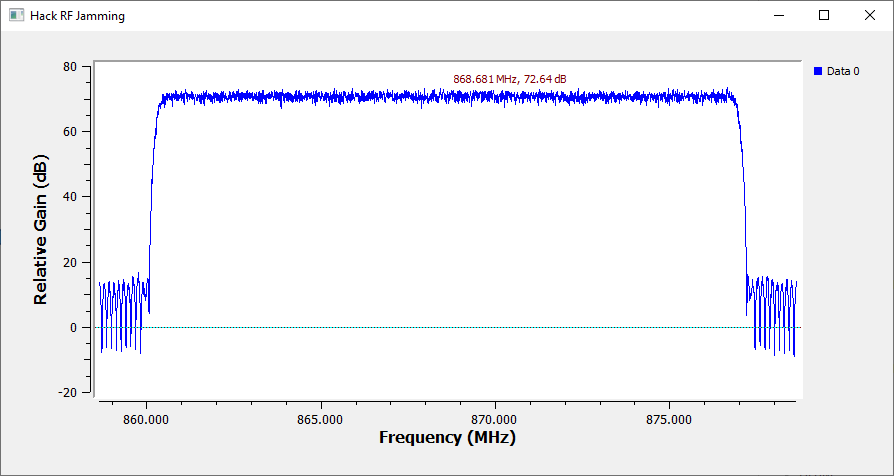
\includegraphics[width=\textwidth]{images/6-pentesting/jamming-output-graph.png}
    \caption{A frequency graph from GnuRadio during the jamming attack.}
    \label{fig:gnuradio-frequency-graph}
\end{figure}

\subsubsection{Results}
This pentest was successful. Signals between the devices were jammed, leaving the system unable to communicate. However, after approximately 60 seconds of running the attack, the main panel triggered an \textit{interference fault event}. While this fault event is triggered and the jamming attack is successfully detected by the system, crucially the event is not logged in the mobile or web application. No notification is sent to the owner of the system whatsoever.

\subsubsection{Discussion}
As expected, the system fails to communicate during the jamming attack. However, the system successfully detects this attack. Arguably, reasonable and appropriate measures have been taken by the manufacturer in this case. Given the inherent vulnerability of jamming attacks in a shared and open medium like radio frequencies, detecting and reporting is the only reasonable course of action 
\cite{optimal-jamming-defense}. This behavior in the system is documented in the official user manual submitted to the FCC \cite{hsgw-user-manual} by Climax Technology. It describes in the \textit{interference} status in section 6.1 of the manual that if a jamming period of 30 seconds or more during a one-minute window is detected then the event is triggered. This lines up with the behavior observed during the test. However, the system fails to log and report the attack to the user. This could potentially let an attacker jam the signal and do a malicious act without the user being notified. Additionally, the parameters of the jamming detection could be questioned. Letting an attacker potentially block \texttt{49\%} of the communication channel might still disturb the system significantly and potentially block important communication.

In this test the most basic jamming technique was used, e.g to send out as much noise as possible at the correct frequency band of as high energy as possible. This makes the attack quite trivial to detect. There exist much more sophisticated jamming attacks, taking less of a brute force approach, which could potentially evade detection and yet still be effective \cite{mpitziopoulos2009survey}. These, however, were considered outside the scope of this test and this report. Additionally, in this test the jamming device (the SDR) was placed very close to the system. In a real world application of this attack, the attacker would be at least a few meters away, blocked by a door. It is doubtful an SDR like the HackRF could generate enough noise to jam the system in those conditions. However, more powerful jammers, using dedicated hardware, could most likely successfully block the systems communication even in those conditions.

\clearpage\section{Task 4: Insecure Network Services} \label{ch:pentesting:network-services}
This section covers the network services found in the system and their implications on the system's security.

\subsubsection{Background}
During development, many manufacturers deploy network services on IoT devices for remote debugging. However, a very common source of vulnerabilities is leaving these network services active on live devices shipped to customers. This could be done in negligence or on purpose to leave a backdoor for the manufacturer to debug live devices. These services could for example be a telnet or SSH server. This combined with weak passwords is an all to common occurrence in IoT systems \cite{understanding-mirai}. This is such a common issue that OWASP ranks it the second most common source of security issues in IoT devices \cite{owasp-iot-top10}.

Often such services are completely unnecessary for the functionality of the system. Even when they are protected by a strong password, which can sometimes be found by analyzing the firmware, other vulnerabilities can be present due to vulnerabilities in the service itself or the OS network stack, as well as outdated versions of said services.

\subsubsection{Method}
Initially, which network services the system hosts had to be found. This was done using the open-source network scanning tool \textit{Nmap}\footnotelink{https://nmap.org/}{2021-05-25}. First the basic port scanning functionality of Nmap was launched against the system, using the following command:
\begin{lstlisting}[frame=tb]
    nmap -p- $IP
\end{lstlisting}
This scans the device for processes listening on all TCP ports in the entire 0-65535 range. Similarly, a scan was made on UDP ports as well. However, due to the known difficultly of UDP port scans, only the most common UDP ports were scanned, as a scan of the full port range was estimated to take several weeks. This was done using the following command:
\begin{lstlisting}[frame=tb]
    sudo nmap -sU -F -v $IP
\end{lstlisting}
The UDP scan showed no active services except a DNS server on port 53. However, the TCP showed three network services listening on different ports on the device. The following network services were identified:
\begin{itemize}
    \item 53/udp: A DNS server.
    \item 53/tcp: A DNS server.
    \item 80/tcp: The local admin server, as described in section \ref{ch:system:local-admin}.
    \item 58098/tcp: An unknown process listening in an unconventional port.
\end{itemize}
The web server listening on port 80 provides very little functionality, as described in section \ref{ch:system:local-admin}. It features a login form. An unsuccessful password attack was conducted against this form, see section \ref{ch:pentesting:password}.

To gain more information about these services a version detection scan was launched against the three ports, using the following command:
\begin{lstlisting}[frame=tb]
    nmap -sV --version-all -p53,80,58098 $IP
\end{lstlisting}
The Nmap version detection scan took around 10 minutes and yielded no result for the unknown application running on port 58098 or any further information about the other two services. To further investigate information about the process the open-source application scanner \textit{Amap}\footnotelink{https://github.com/BlackArch/amap}{2021-05-26} was used. This is a lesser known program created by the prolific hacker group \textit{The Hacker's Choice}\footnotelink{https://www.thc.org/}{2021-05-26}. According to the authors, the Amap application scanner has largely been superseded by Nmap. However, the application suite includes a very simple TCP fuzzer called \textit{Amapcrap}. This is a program that sends random bytes to an open TCP port to illicit a response from an otherwise silent application, which can be very useful in black box testing an opaque network service. This was tried against the system using the following command:
\begin{lstlisting}[frame=tb]
    amapcrap $IP 58098
\end{lstlisting}

\subsubsection{Results}
The result of the full port scan shows three active services on the device:
\begin{itemize}
    \item A DNS server, running on the standard DNS ports of \textit{53/tcp} and \textit{53/udp}.
    \item A web server, \textit{80/tcp}, the functionality of which is covered in section \ref{ch:system:local-admin}.
    \item An unknown application, running on \textit{58098/tcp}.
\end{itemize}
Additionally, the application and version scanners which were run against the services gave no information at all about the three services.

Lastly, fuzzing the unknown service (\textit{58098/tcp}) made the service unresponsive, as shown in figure \ref{fig:amapcrap-fuzz-attack}. Presumably, the application crashed on this specific input.
\begin{figure}[!ht]
    \centering
    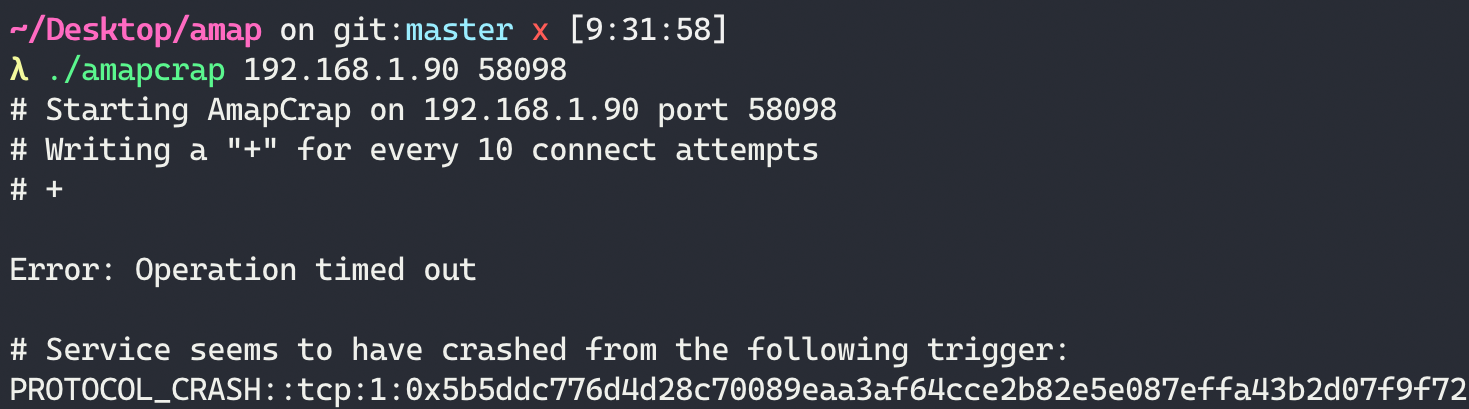
\includegraphics[width=\textwidth]{images/6-pentesting/amapcrap-fuzz-crash.png}
    \caption{The 58098/tcp application crashing during a fuzzing attack.}
    \label{fig:amapcrap-fuzz-attack}
\end{figure}
Examining the input further reveals that the first two bytes represent the characters \texttt{[]} in ASCII, which is interesting. Through manual testing and trial and error over telnet it was discovered that the application crashed on more inputs, including \texttt{\{\}} and \texttt{[1,2,3]}. While the application presumably crashes and becomes temporarily unresponsive, the system seems to revive the process and within about a minute it starts accepting TCP connections again.

\subsubsection{Discussion}
Performing a network scan on the system revealed three network services listening on three different TCP ports. However, no vulnerabilities were found as a result of these three services. The purpose of the first one, the DNS server, is quite unclear. There is seemingly no self-hosted domain documented anywhere so why the system hosts a DNS server is as of now unknown. The second server, the HTTP web server, has been covered at length in section \ref{ch:system:local-admin}, as well as a pentest that was launched against it which is covered in section \ref{ch:pentesting:password}. The third server is the most interesting find from this section. It is hosted on an unconventional TCP port, presumably to hide it slightly from attackers. The application is completely opaque and does not seem to react at all to most inputs. Through all fuzzing and manual testing the application never sent a single response over the TCP connection. However, though fuzzing several inputs were found that seemingly crash the server. The pattern in the inputs suggests that the server might be trying to parse JSON and crashing when the input is of an unexpected format.

A guess as to the functionality of this server is an obfuscated backdoor to the server. Instead of a standard telnet server it might be hidden behind an application that expects a specific string. Only when it receives it does the remote shell launch. However, as it stands currently the application is a complete black box. Without access to the firmware additional investigation is very difficult. It was therefore considered unfeasible and it was not investigated further.

As stated, no additional vulnerabilities were discovered as a result of this investigation into the systems network services. The more important question, however, is \textit{why}? When OWASP ranks it as the second most common source of security issues for this type of system \cite{owasp-iot-top10}, why are these network services active on the device in the first place? There is seemingly no reason for them to exist. If one were to discover the password to the admin web panel, for example, every aspect of the security of the system is compromised. It opens up the system to potentially critical vulnerabilities. Climax Technology have already made this mistake at least once before. Researchers investigating a similar system from the same manufacturer discovered a telnet server listening on a similar unconventional high port. By analyzing the firmware they found that the root password could be derived simply from the panels MAC address \cite{labvienna} (see section \ref{ch:related-work:lupus}), giving them complete control over the system. Unfortunately, the firmware to the system in this thesis was not found publicly available. It was decided to be outside the scope of this thesis but if one were to, for example, solder off the flash memory from the main panel's PCB and read it's contents one could get access to the firmware. It is not unlikely that through reverse engineering the firmware one could find the password to the local admin panel or understand more about how the \textit{58098/tcp} application works and what its purpose is. This could lead to additional severe vulnerabilities. The fact is that these services are seemingly not needed for the functionality of the system and only serve to increase the attack surface of the system.

\clearpage\section{Task 2: Online Password Attack} \label{ch:pentesting:password}
An online password attack refers to probing an active login, as opposed to an offline attack where you for example might try to crack a hash of a leaked database. This attack involves using some type of approach to test many passwords of a login form to try and find valid credentials. The local web admin page (see section \ref{ch:system}) has a login page that could potentially be brute-forced.

\subsubsection{Background}
A password attack, or password cracking, refers to cyber-attacks where the attacker tries to figure out valid credentials, to gain authorized access to a system. These can be categorized into two groups: offline and online password attacks. The former refers to attacks requiring no communication with the system in order to test a valid password. An example could be listening in on network traffic and seeing a password hash. One could then perform an offline password attack by trying to figure out which password produced that hash, and thus login to the system. In an online attack, the system under attack is in continuous communication with the attacker. This could be, for example, writing a script to try many different passwords on a login page of a web page. Online password attacks are generally harder to successfully perform. They are often much slower, as the communication with the system incurs a major overhead, and also poses the potential risk of getting caught in the middle of it if the administrator of the system notices the malicious traffic. Servers also often implement rate-limiting against IP addresses to combat these types of attacks and DOS attacks.

For both online and offline password attacks, there are several techniques one can use to try and guess the correct password. The simplest one is a \textit{brute-force attack}, where the attacker simply tries all possible passwords up to some length. Given $c$ possible characters in the password and a password length of $l$, there are $c^l$ possible passwords to try. This has exponential complexity in the length of the password, and will thus scale very poorly with longer passwords. Another technique is called a \textit{dictionary attack}, where the attacker uses a large list of known common passwords. Often these lists are created from actual passwords from leaked databases. For offline attacks like hash-cracking, there are additional techniques like \textit{rainbow tables}.

In the case of the system in this thesis, we have no opportunity for an offline password attack, as no information about the password such as a hash is leaked as far as the author is aware. The local admin web page does, however, feature a login page. This page uses \textit{HTTP Basic authentication} to log in to the main panel (see figure \ref{fig:local-login-page}). If this login system has not implemented any form of rate-limiting then guessing the right password might be possible, given enough time and resources.

\subsubsection{Method}
We know from sources like the one covered in section \ref{ch:related-work:lupus} that \textit{admin} is most likely a valid user name. This is further indicated by the official user manual from Climax Technology\footnotelink{https://fccid.io/GX9HSGWF1919/Users-Manual/Users-Manual-4873123}{2021-04-22}, which includes default login credentials with the admin user name (the credentials do not work on this system). As stated, the login form (see figure \ref{fig:local-login-page}) uses \textit{HTTP Basic authentication} to authenticate the user. A dictionary attack was performed against this login page. The well-known password list \textit{rockyou.txt}\footnotelink{https://github.com/danielmiessler/SecLists/blob/master/Passwords/Leaked-Databases/rockyou-20.txt}{2021-04-25} was used as the dictionary. A useful program to perform online password attacks is called \textit{Hydra}\footnotelink{https://github.com/vanhauser-thc/thc-hydra}{2021-04-21}, which is a command-line tool. Using the following command, Hydra was used to perform the attack:
\begin{lstlisting}[frame=tb]
    hydra -l admin       \
          -P rockyou.txt \
          192.160.1.90   \
          http-get       \
          "/action/login:F=Access Denied"
\end{lstlisting}

\subsubsection{Results}
The test was mostly unsuccessful. A password attack against the system was successfully executed. However, Hydra only manages to perform around 23 requests per minute against the main panel, see figure \ref{fig:hydra-password-attack}. This is too slow to be able to guess enough passwords to have a meaningful probability at a correct guess.
\begin{figure}[!ht]
    \centering
    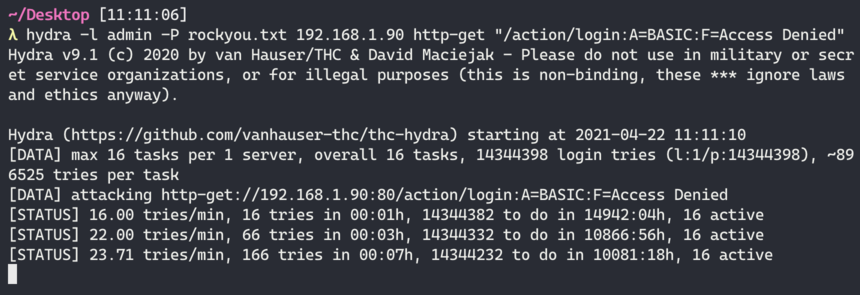
\includegraphics[width=\textwidth]{images/6-pentesting/hydra-results.png}
    \caption{The results of running a password attack.}
    \label{fig:hydra-password-attack}
\end{figure}

\subsubsection{Discussion}
The Hydra tool was only able to do around 23 requests per minute. Hydra is known to be very fast, so that is not the issue. One explanation for why this was so slow could be that the server rate-limits users. This is a common technique to protect against password attacks, if enough failed login attempts occur from a single IP the server would temporarily block or throttle it. However, there are signs indicating that this is not the case. For example, accessing the main web page slows down tremendously while performing the attack. Initially, it had around a \textit{16ms} response time, which increased to over \textit{17 seconds} during the attack. This was even confirmed on another computer, indicating that the main panel has not implemented any form rate-limiting per IP address. Presumably, the system is instead simply resource-bound and cannot serve requests at a faster rate. Given the hardware of the system, this is not unlikely. The CPU is most likely not that powerful, as is often the case in \gls{IOT} systems.

Due to the main panel not being able to serve more than 23 requests per minute, this type of attack is not feasible. For example, running a brute force attack, testing just all possible eight-character passwords, would take well over a hundred thousand years. A well-crafted dictionary attack could perhaps be effective, even at these slow speeds. However, there is some indication that the password might be just a random string of characters, given that the default password cited in the user manual is \texttt{cX+HsA*7F1}. If that is the case then a brute force technique is the only possibility. For these reasons, the attack was deemed unfeasible and not pursued further.

\clearpage\section{Task 3: Climax Technology's Vesta platform} \label{ch:pentesting:vesta}
Climax Technology, the manufacturer of the hardware used in this system, does not seem to be a consumer-facing business. Nonetheless, they have their own software platform to control their system, called \textit{Vesta}. In the SecuritasHome system, this platform and its components are essentially replaced by \textit{Alarm.com}. The Vesta platform features a mobile application\footnotelink{https://play.google.com/store/apps/details?id=com.climax.vestasmarthome.eu}{2021-04-20} to control the system, as well as a web portal\footnotelink{https://eu.vestasmarthome.com/Vesta/}{2021-04-20}. A potential security vulnerability is if this Vesta platform is still active and usable to control this system.

\subsubsection{Background}
As stated above, Climax Technology have their own platform, branded as Vesta, to control the system. A common vulnerability in IoT devices is not covering up vulnerabilities arising higher up in the supply chain (\todo source). In this system, there is a possibility that \textit{Alarm.com} has not properly deactivated the access and functionality of the Vesta platform. The idea is for the Alarm.com platform to replace it entirely.

In the app \textit{Vesta Home 5 EU}, see figure \ref{fig:vesta-home-app}, one can perform essentially all actions that the Alarm.com mobile application provides (see section \ref{ch:system:software}). On the landing page, you are greeted with simple a login page (where your Alarm.com credentials don't work). However, it also includes a button labeled \textit{First Time Registration} (see figure \ref{fig:vesta-landing-page}), where one can register a new account connected to a new system. To register a new system one only needs to enter its MAC address, see \ref{fig:vesta-registration-page}, which is available without authorization from the local admin page (see \ref{ch:system:software}). Potentially, one could then register the system in the Vesta platform to gain authorization to control the system, thus bypassing the security completely.
\begin{figure}[!ht]
    \centering
    \begin{subfigure}[t]{0.4\textwidth}
        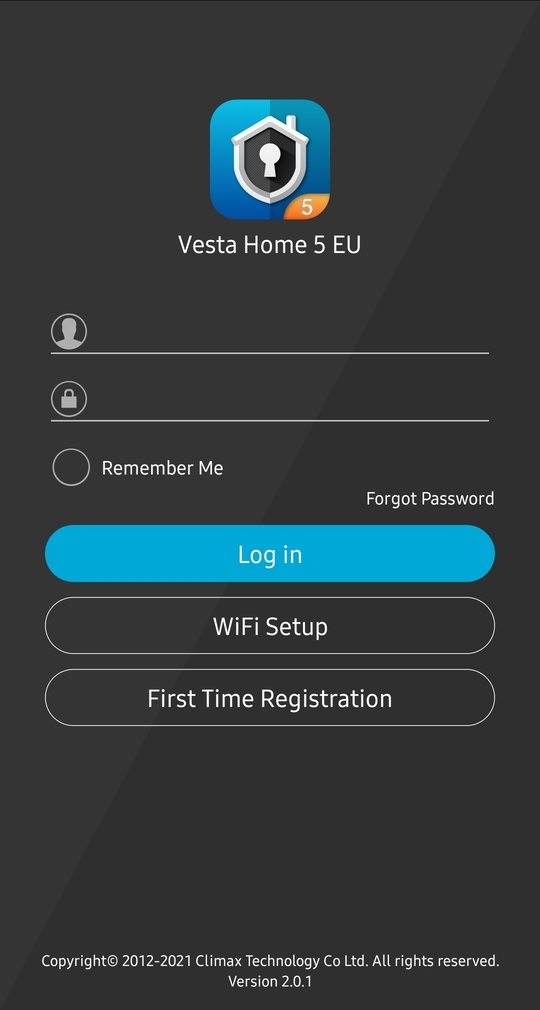
\includegraphics[height=3.8in]{images/6-pentesting/vesta-home-landing-page.jpg}
        \caption{The landing page}
        \label{fig:vesta-landing-page}
    \end{subfigure}%
    ~
    \begin{subfigure}[t]{0.4\textwidth}
        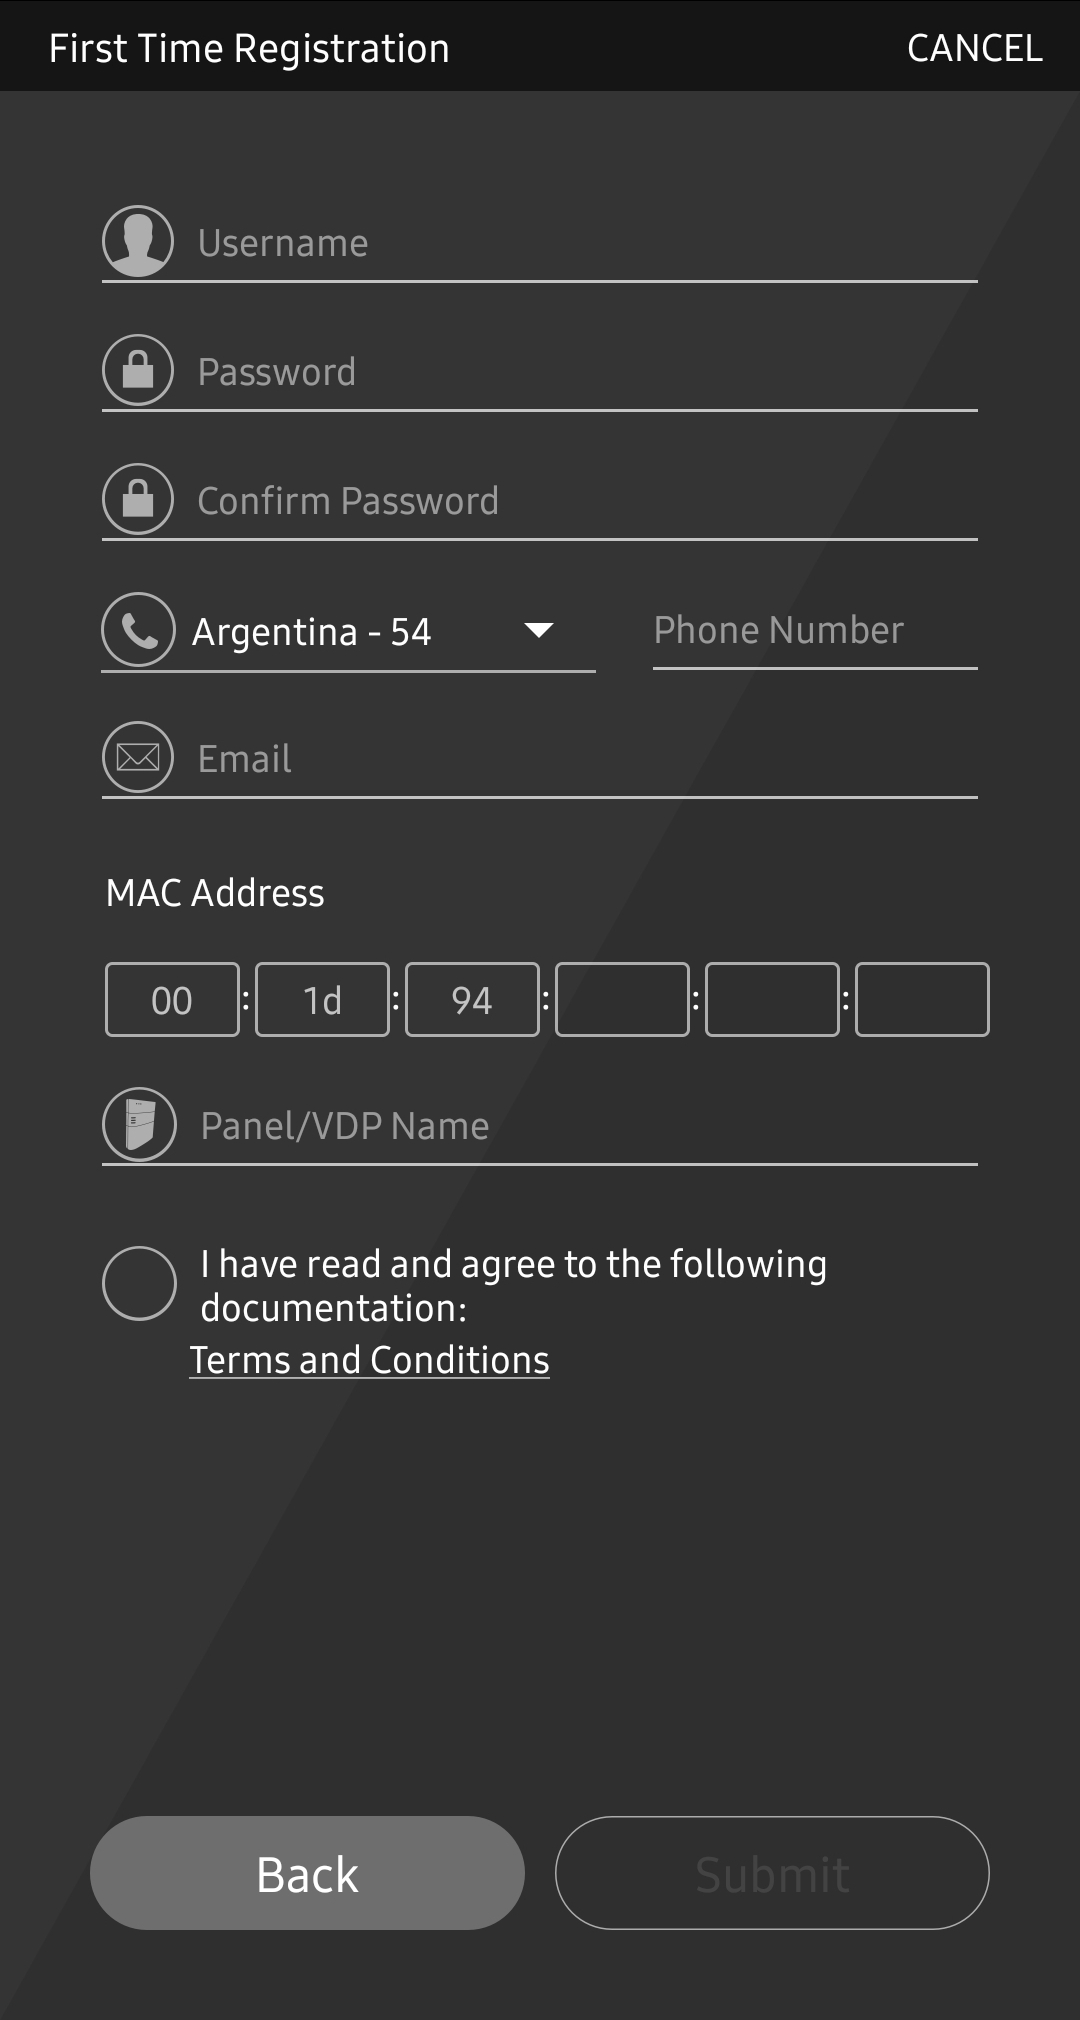
\includegraphics[height=3.8in]{images/6-pentesting/vesta-home-registration.jpg}
        \caption{The "First Time Registration" page}
        \label{fig:vesta-registration-page}
    \end{subfigure}
    \caption{The Vesta Home 5 EU mobile application.}
    \label{fig:vesta-home-app}
\end{figure}
In the Vesta web application, there is a very similar form, allowing you to register a new device using the MAC address, see figure \ref{fig:vesta-web-registration}.
\begin{figure}[!ht]
    \centering
    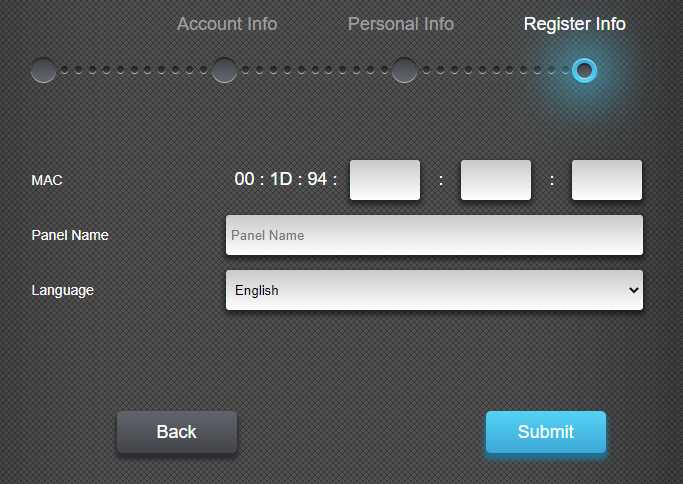
\includegraphics[width=0.9\textwidth]{images/6-pentesting/vesta-web-registration.png}
    \caption{The Vesta web application registration.}
    \label{fig:vesta-web-registration}
\end{figure}

\subsubsection{Method}
The mobile application is free to download. To be able to confidently monitor the network traffic, the mobile application was installed on an android emulator for PC, and Wireshark was run on the host machine.

Both applications use HTTPS, meaning the requests are encrypted. An attempt was made to perform a \gls{MITM} attack on the mobile application to view the HTTPS traffic, using \textit{mitmproxy}\footnotelink{https://mitmproxy.org/}{2021-04-21} and the built-in proxy settings of the android emulator. However, this made the application yield an error message saying it could not reach the server. Presumably, the application uses certification pinning to protect against this type of attack. This was not explored further since the traffic can easily be viewed in the web application, using the Chrome network tab (see figure \ref{fig:vesta-web-registration-failed}), and most likely both applications access the same API.

\subsubsection{Results}
The penetration test was unsuccessful. Both the mobile application and the web application yielded identical results. A simple error message is shown, saying the \textit{MAC/IMEI} is incorrect, see figures \ref{fig:vesta-home-registration-failed} and \ref{fig:vesta-web-registration-failed}. In the Chrome network tab, we can see when trying to register the system through the web application that the API responds with the message "no data found!".
\begin{figure}[!ht]
    \centering
    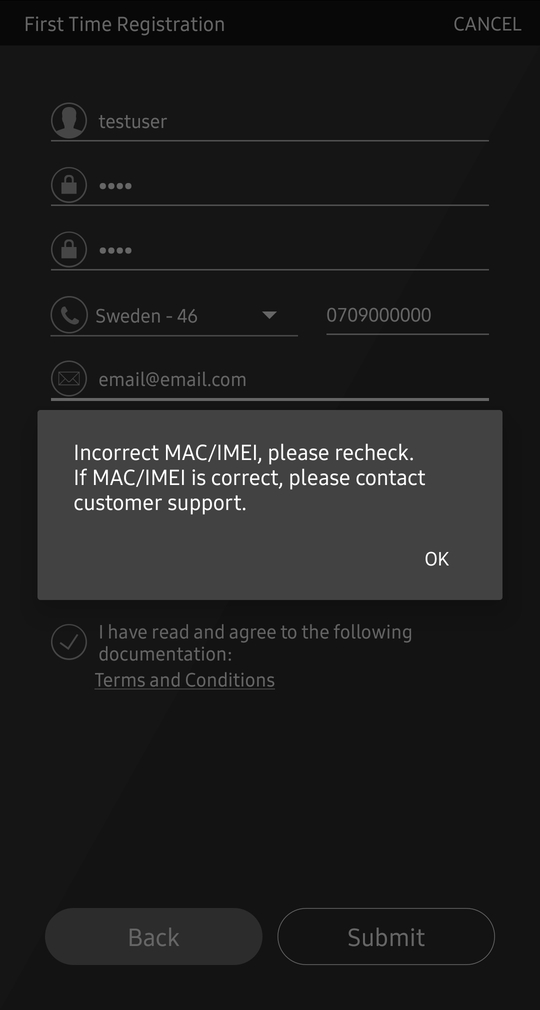
\includegraphics[width=0.4\textwidth]{images/6-pentesting/vesta-home-registration-failed.jpg}
    \caption{The results of trying to register in the Vesta mobile app.}
    \label{fig:vesta-home-registration-failed}
\end{figure}
\begin{figure}[!ht]
    \centering
    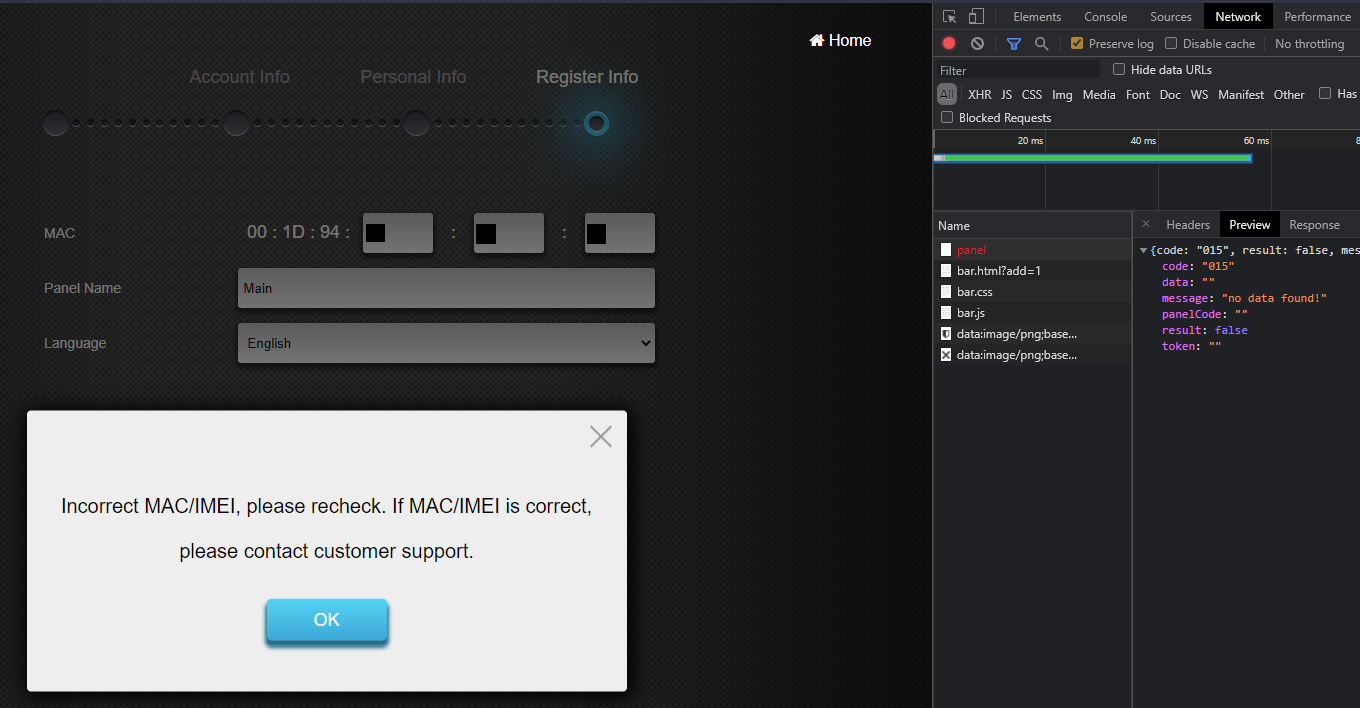
\includegraphics[width=0.9\textwidth]{images/6-pentesting/vesta-web-registration-failed.png}
    \caption{The results of trying to register in the Vesta web app.}
    \label{fig:vesta-web-registration-failed}
\end{figure}

\subsubsection{Discussion}
Trying to register the hardware to the Vesta platform was unsuccessful. The given MAC address was not accepted. Presumably, Climax Technology has a database of the MAC addresses of all sold systems under the Vesta platform. While the MAC address of the system in this thesis is registered under Climax Technology, it does not seem to be registered by the Vesta platform. Another possibility is that the MAC address and IMEI number pair is not registered because \textit{Alarm.com} has used their own SIM cards and thus a different IMEI number. This is indicated by the error messages shown. Which of these scenarios is the correct one, we cannot know. Either way, we can see that the API responds with a negative result, saying that no data could be found. Therefore, this type of supply chain error seems to have been identified and correctly protected against.

\clearpage\section{Task 4: Insecure default credentials}
This section covers the topic of insecure default credentials. It does not include a \textit{pentest}, per se, but instead a list of all such credentials discovered in the system. These were discovered during the exploratory phase, and threat modeling phase of the project. Therefore, this section does not include a method part.

\subsubsection{Background}
Often default credentials are unavoidable. When first accessing the system, you need some way to do that without having authenticated yourself before. These credentials can, however, be more or less secure. A huge problem within cybersecurity is using insecure default credentials that can be easily guessed by a hacker. Additionally, often the user is never forced or even encouraged to change these credentials, leading to a potentially severe vulnerability. A common example is routers, which almost always feature an admin page to configure settings. Usually, all routers of the same model have the same default login credentials and often these are as simple as \texttt{admin:admin}. This is such a common issue that there are public databases of these passwords for each model \footnotelink{www.routerpasswords.com}{2021-0501}. Often the owner of the router is not even aware that this page exists or that they should change the password.

Famously, the MIRAI botnet relied on insecure default credentials to hack into hundreds of thousands of devices. It used just \texttt{62} different credentials \cite{understanding-mirai}. MIRAI is a worm malware, which targeted mostly IoT devices. It looked for devices with TCP port 23 or 2323 open, which are both often used by Telnet, and tried these credentials there. After gaining successful authentication against the device, these credentials and IP would be sent to a central server. Using this technique, over half a million devices were hacked and incorporated into the MIRAI botnet, which in turn was able to perform large scale DDOS attacks against websites. It was able to reach almost \texttt{1 TB/s} against a single target.

\subsubsection{Results}
The system can be armed and disarmed via the remote keypad (see section \ref{fig:hardware-components}) by entering a personal four-digit pin. By default, this is set to \texttt{1234}. You are never forced or even encouraged to enter a new code, overriding the easily-guessable default.

Additionally, when an alarm is triggered Securitas will send security personnel to inspect the site. If you accidentally triggered the alarm yourself Securitas has a phone number you can call to cancel the alarm. However, as a security mechanism, when doing this you have to correctly say a four-digit code (different from the previously discussed code). If you do not remember your code or say it incorrectly personnel will be sent to the site regardless. This code is by default the last four digits of \textit{your phone number}. Once again, you are never forced or even encouraged by the system to change this code.

No other bad default credentials were found. Importantly, the local admin panel (see section \ref{ch:system:software}) does not seem to use bad default credentials. Several hundred common default passwords were tried and none of them were successful (see section \ref{ch:pentesting:password}).

\subsubsection{Discussion}
Two insecure default credentials were discovered in the system. The first one, the arming pin defaulting to \texttt{1234}, is relatively severe. After triggering an alarm, you have a set time interval to disable it using your personal four-digit pin before the alarm is sent to the alarm center. An attacker could bet on the fact that this code has not been changed, and use it to turn off an alarm after breaking into the house. One could argue, however, that the probability of someone not changing this code is relatively low. The code arguably has an \textit{obvious} insecurity, leading to people perhaps feeling a greater need to change it. However, using a random code as the default would be substantially more secure.

The second code, used to call off an active alarm, is also a security issue. Your address and phone number can often easily be tied to one another and looked up using publicly available resources. An attacker obviously has the address if they are trying to get access to the house. Finding the phone number of the resident could be done in seconds using public websites for example. However, people can have multiple phone numbers and the house can of course have multiple residents.

Both identified insecure default credentials require the attacker to take quite a big risk to be able to exploit. An attacker would have to break into a house and only afterward bet on the fact that these had not been changed. One could then either turn off the alarm or try and call the alarm central before the owner does. All while the owner has been notified of an alarm breach via both email and the mobile app (see section \ref{ch:system:software}). While perhaps not critical vulnerabilities, they are nevertheless completely unnecessary. The system could easily give you a random code instead or force you to enter one upon first registering the system. Giving it an insecure default or tying it to publicly available information is not ideal and can be easily avoided.

